\section{落下間隔変化における高速化への寄与}
\subsection{落下実験結果}

容器Bにおいて落下間隔を5分,10分,20分と変化し,球を落下させた解析した結果をFig.\ref{fig:falling-5},\ref{fig:falling-10},\ref{fig:falling-20},に示す.縦軸は落下速度,横軸は落下開始時からの経過時間である.なお,落下間隔10分の結果に関して,比較のため先行研究であるIwamuro\cite{ref:9}における実験結果もあわせて示す.それぞれの場合において,超音波照射による落下球の高速化は見られた.

しかし,Iwamuro\cite{ref:9}と比較し,落下開始時の加速におけるオーバーシュートが今回は見られなかった.また,Iwamuro\cite{ref:9}においては落下速度は落下開始から0.8s以降,定常状態となっている.本実験において同条件である落下間隔10分において,超音波照射なしの場合,落下開始から0.2-0.7s間のみ,一定速度で落下し以降は加速した.オーバーシュートの有無は先述の装置改良における実験結果においても見られたため,実験手法の変化によるためだと考えられる.終端速度への到達の有無だが,擬塑性流体の粘弾性回復がIwamuro\cite{ref:9}と比較して十分に行われていないと考えられる.これは,落下間隔20分の条件において,Iwamuro\cite{ref:9}と同様の終端速度に達しているため,落下間隔10分では回復しきれなかった粘弾性が回復しきったためだと考えられる.粘弾性の回復時間が異なることに関しては,落下間隔をより細かく変化させ調査する必要があると考えられる.

\begin{figure}[ht]
    \centering
    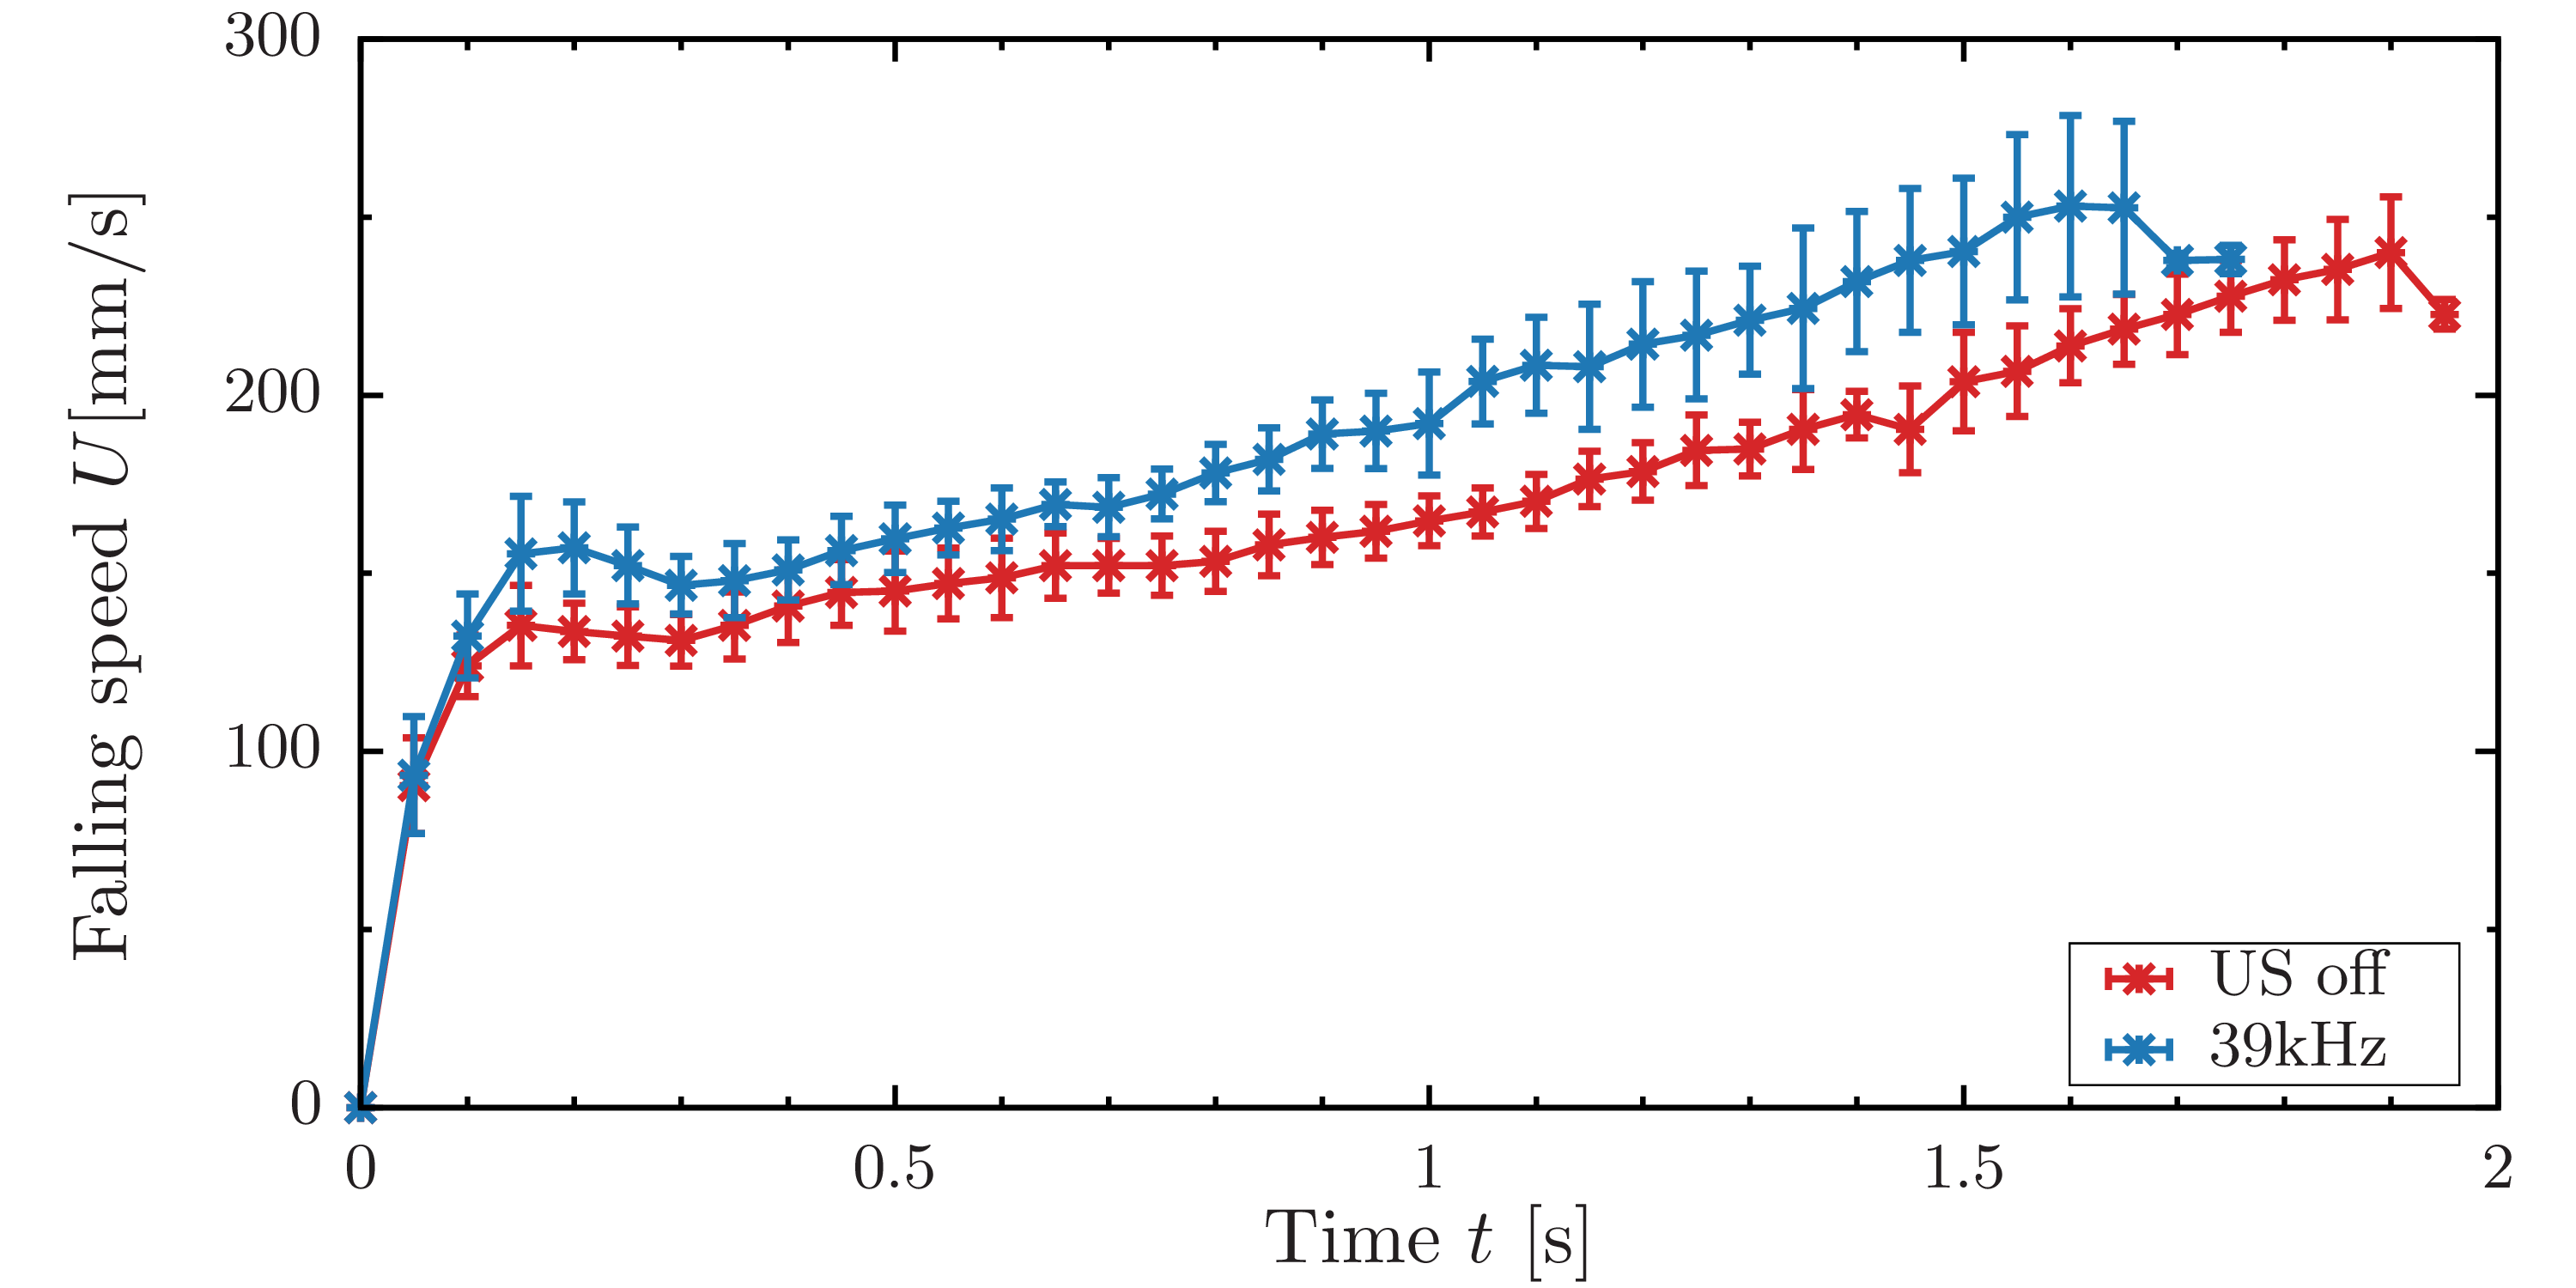
\includegraphics[width=11cm,clip]{./4-Results/s1-5.png}
    \caption{Falling velocity of a sphere in 1wt.\%PAA solution with and without ultrasound irradiationin tank B. (Interval 5 min.)}
    \label{fig:falling-5}
\end{figure}
\begin{figure}[ht]
    \centering
    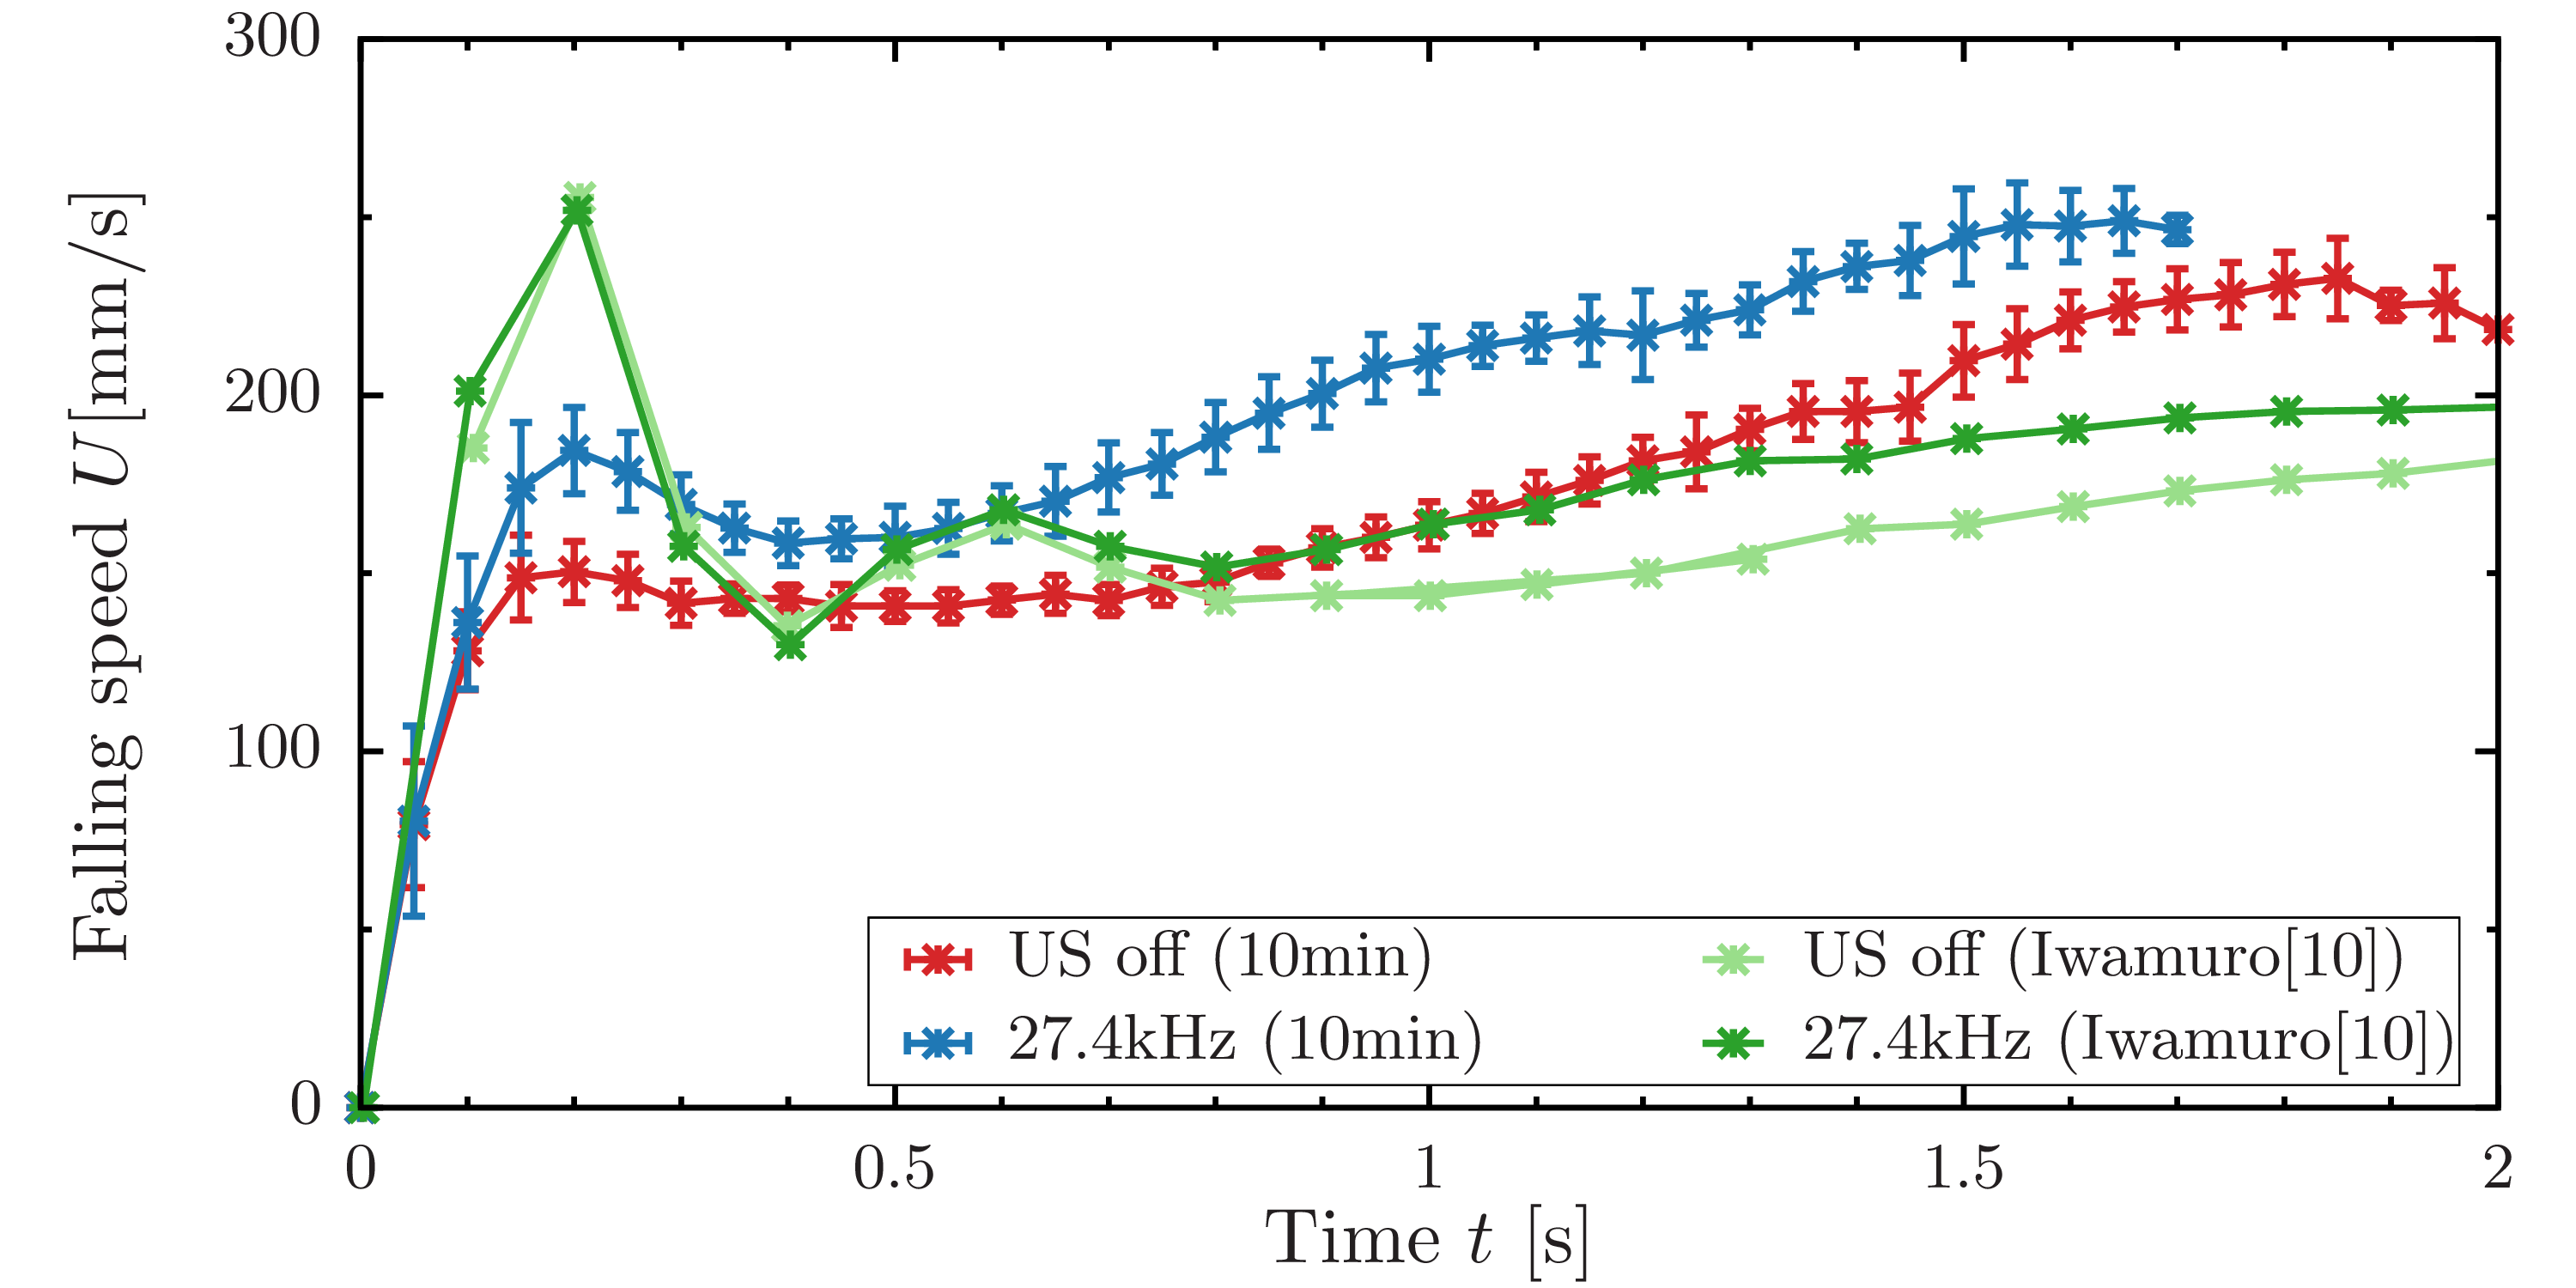
\includegraphics[width=11cm,clip]{./4-Results/s1-10.png}
    \caption{Falling velocity of a sphere in 1wt.\%PAA solution with and without ultrasound irradiationin tank B. (Interval 10 min.)}
    \label{fig:falling-10}
\end{figure}
\begin{figure}[ht]
    \centering
    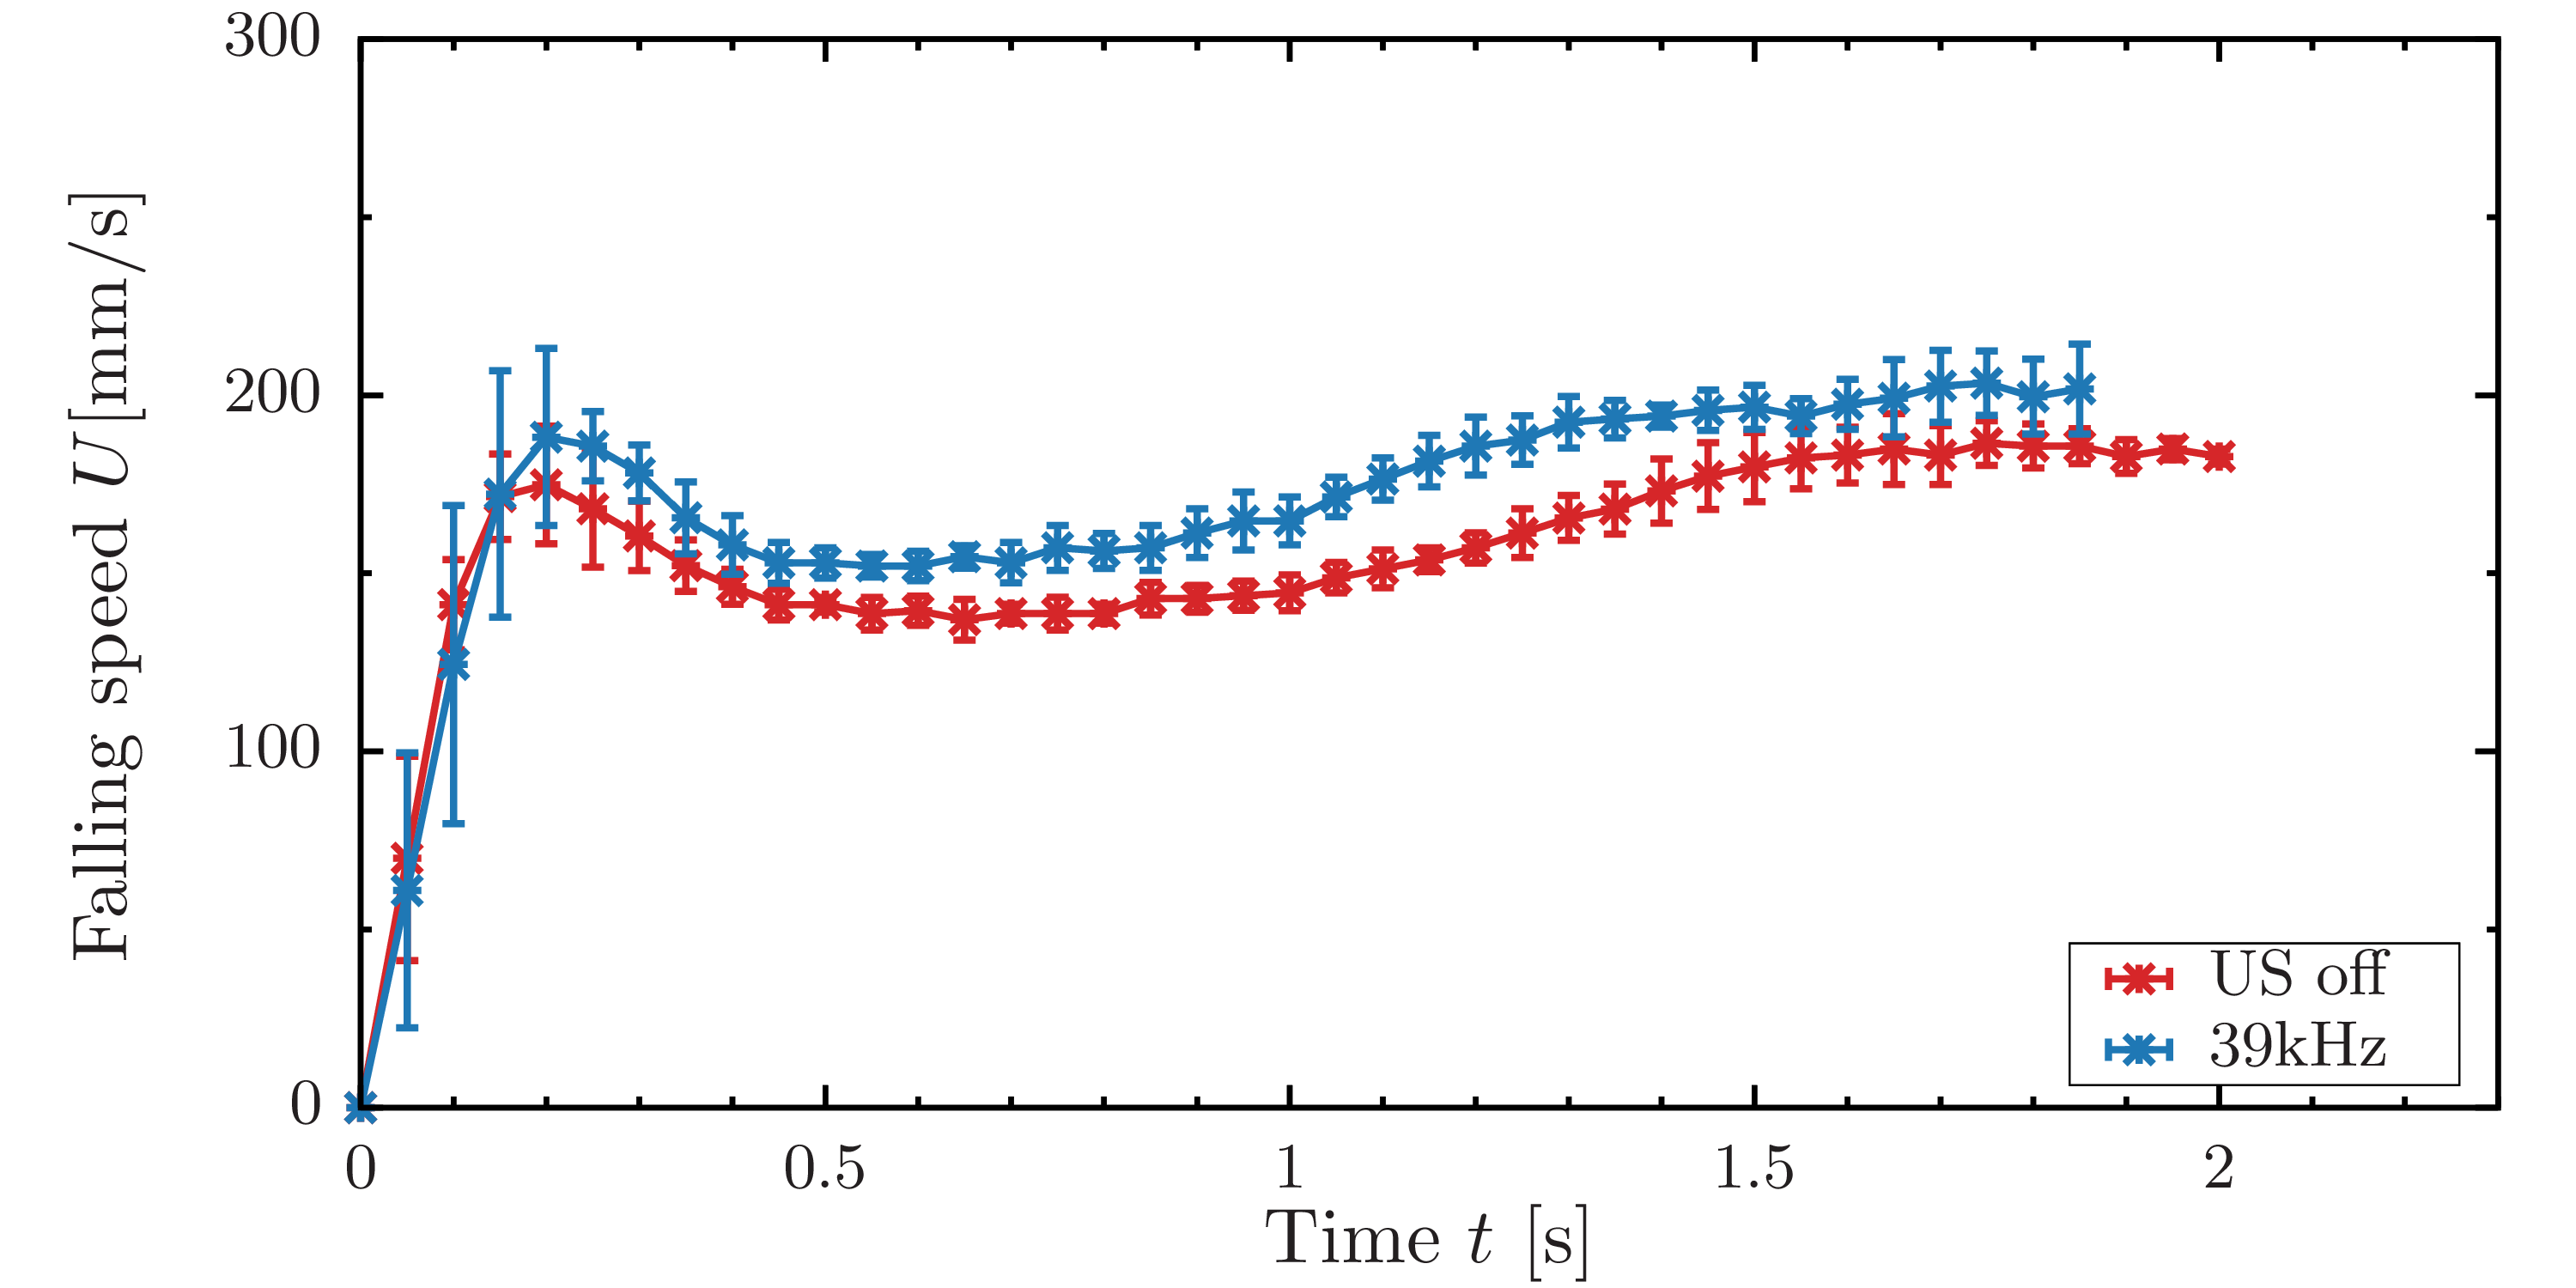
\includegraphics[width=11cm,clip]{./4-Results/s1-20.png}
    \caption{Falling velocity of a sphere in 1wt.\%PAA solution with and without ultrasound irradiationin tank B. (Interval 20 min.)}
    \label{fig:falling-20}
\end{figure}

\subsection{超音波照射による高速化}

球の落下間隔を5分,10分,20分と変化させた.その結果をFig.\ref{fig:interval-change}に示す.なお,縦軸は落下速度[mm/s],横軸は落下開始時からの経過時間[s]である.全ての条件において超音波照射に伴う高速化は見られた.また落下速度は,落下間隔10分,5分,20分の順で速かった.この結果を元に,超音波照射時の球の落下速度$U_{on}$と超音波照射なしの球の落下速度$U_{off}$として,速度比$U_{on}/U_{off}$を求めた.その結果をFig.\ref{fig:speed-diff}に示す.ここで縦軸は速度比[-],横軸は落下間隔時間[min]である.この結果より,落下速度と同様に,落下間隔10分,5分,20分の順で超音波照射による高速化が見られた.このことに関して,超音波照射による高速化のメカニズムより考える.

擬塑性流体中を落下する球に伴う,慣性,粘性の影響に関して考えるため,レイノルズ数の計算を行う.式\ref{eq:power-low}のPower-law modelが適用できる流体中における粒子のレイノルズ数は,
\begin{eqnarray}
    Re = \frac{\rho_1 \left(2a\right)^n U_T^{2-n}}{k} ,
\end{eqnarray}
と表される\cite{ref:1,ref:8-5}.今回の実験結果より,$\rho \approx$1000[kg/m${}^3$],$2a =$0.01[m],$U_T \approx$0.2[m/s],\\$k =$8.37[Pa$\cdot \text{s}^n]$,$n =$0.24であるので,$Re \approx$2.3と概算することができる.これより,粒子付近の流れはストークス流れに従い,粘性が支配的であると考えられる.

本研究の系は,一様流れ中を半径$a$の球および,超音波の伝播が存在する系である.超音波の伝播に関して,音波の圧力変動の時間スケールは$O\left(10^{-5}\right)$sである.一方で,球の落下時間スケールは$O\left(10^{0}\right)$sとなるため,圧力変動の時間スケールは非常に短い.このことより,球の落下に関して平均的な挙動に着目することで音波の伝播に伴う圧力変動の非定常性を無視することができる.球周囲に存在する非圧縮性流体の単位体積の運動方程式について考える.球によって誘起される応力テンソルを$\bm{\sigma}$,流体の密度を$\rho$,速度ベクトルを$\bm{v}$,体積力を$\bm{X}$とすると,
\begin{eqnarray}
    \rho \frac{D\bm{v}}{Dt} = \bm{X} + \nabla \cdot \bm{\sigma} ,
    \label{eq:undou}
\end{eqnarray}
となる.また,非圧縮性流体を仮定しているため連続の式が成り立つ.
\begin{eqnarray}
    \nabla \cdot \bm{v} = 0 .
    \label{eq:renzoku}
\end{eqnarray}
式\ref{eq:renzoku}より,式\ref{eq:undou}の左辺は,
\begin{eqnarray}
    \rho \frac{D\bm{v}}{Dt} = \frac{\partial \bm{v}}{\partial t} + \left(\bm{v} \cdot \nabla \right) \bm{v} ,
    \label{eq:nabie}
\end{eqnarray}
と展開できる.流れは十分に発達し,定常状態であると仮定することで,式\ref{eq:nabie}の右辺第1項の時間微分項は0となる.低レイノルズ数かつStokes近似を用いることにより,慣性項は粘性項より十分に小さいと仮定することができる.これにより,式\ref{eq:nabie}の右辺第2項の慣性項は無視することができる.加えて,周囲の流体において密度差が存在しないので,体積力$\bm{X}$は0となる.これらより,式\ref{eq:undou},\ref{eq:nabie}を用いると,
\begin{eqnarray}
    \nabla \cdot \sigma = 0 ,
    \label{eq:sigma-}
\end{eqnarray}
といった関係が導かれる.

ある球体領域において,ガウスの発散定理より,
\begin{eqnarray}
    \int_S{\bm{\sigma \cdot \bm{n}}}dS = \int_V{\nabla \cdot \bm{\sigma}}dV ,
    \label{eq:gaussian}
\end{eqnarray}
といった関係が成り立つ.ここで,$\bm{n}$は球領域表面に対する法線ベクトル,$S$は球の表面積,$V$は球の体積を表す.式\ref{eq:sigma-}より,式\ref{eq:gaussian}は定数となることが分かる.式\ref{eq:sigma-},\ref{eq:gaussian}は任意の流体体積に関して成り立つため,球の表面($r = a$)と球外部の任意の領域($r > a$)において,以下の関係が成り立つ.
\begin{eqnarray}
    \int_{r=a}\bm{\sigma}\cdot\bm{e}_r dS=\int_r\bm{\sigma}\cdot\bm{e}_r dS .
    \label{eq:inte}
\end{eqnarray}
ここで,$\bm{n} = \bm{e}_r$とする.この式は,任意の領域において,面積力が釣り合うことを示す.$r = a$における時間平均応力を$\langle\sigma\rangle_a$,$r$における時間平均応力を$\langle\sigma\rangle_r$とそれぞれする.球の表面積$S=4\pi r^2$であるので,式\ref{eq:inte}は,
\begin{eqnarray}
    4\pi a^2\langle\sigma\rangle_a = 4\pi r^2\langle\sigma\rangle_r ,
    \label{eq:sigma1}
\end{eqnarray}
となる.球表面において,球の体積力と表面力は釣り合うので,
\begin{eqnarray}
    4\pi a^2\langle\sigma\rangle_a = \frac{4}{3} \pi a^3 \Delta \rho g ,
    \label{eq:sigma2}
\end{eqnarray}
となる.ここで,球と流体の密度差$\Delta \rho$,重力加速度$g$である.式\ref{eq:sigma1},\ref{eq:sigma2}より,
\begin{eqnarray}
    \langle\sigma\rangle_r = \frac{a^3\Delta\rho g}{3r^2} ,
\end{eqnarray}
となる.低レイノルズ数で粘性項が支配的であるため,
\begin{eqnarray}
    \langle\sigma\rangle_r \sim \mu \dot{\gamma} ,
    \label{eq:sigma3}
\end{eqnarray}
と概算することができる.Power-law modelが適用できる領域での議論を行っているため,式\ref{eq:power-low},\ref{eq:sigma3}より,
\begin{eqnarray}
    \dot{\gamma} \sim \left(\frac{a^3\Delta\rho g}{3r^2 k}\right)^{\frac{1}{n}} ,
    \label{eq:gamma_abs}
\end{eqnarray}
と概算される.この系において,エネルギー散逸に関して考える.位置エネルギーと粘性によるエネルギー散逸が釣り合うため,単位時間あたりに系全体が失うエネルギーバランスより,以下の式が成立する.
\begin{eqnarray}
    \int_{r>a}\bar{\epsilon}dV = 4 \pi \int^\infty_a \bar{\epsilon}r^2 dr = \frac{4}{3}\pi a^3\Delta\rho g U_T ,
    \label{eq:eg}
\end{eqnarray}
ここで,$U_T$は球の終端速度,$\bar{\epsilon}$は時間平均された単位体積当たりのエネルギー散逸である.また,粘性散逸$\bar{\epsilon}$は,以下の様に概算される.
\begin{eqnarray}
    \bar{\epsilon} \sim \langle\sigma\rangle_r\dot{\gamma} \sim \mu \dot{\gamma}^2 \sim \frac{\langle\sigma\rangle_r^2}{\mu} ,
    \label{eq:eps}
\end{eqnarray}
式\ref{eq:sigma3},\ref{eq:eg},\ref{eq:eps}より,終端速度は
\begin{eqnarray}
    U_T \sim \frac{a^3\Delta\rho g}{3}\int_a^\infty\frac{dr}{\mu r^2} ,
    \label{eq:UT0}
\end{eqnarray}
と見積もられる.式\ref{eq:power-low},\ref{eq:gamma_abs},\ref{eq:UT0}より,終端速度は下記の様に書き直される.
\begin{eqnarray}
    U_T \sim \frac{a^3\Delta\rho g}{3}  \int^{\infty}_{a} \frac{dr}{\mu r^2} \sim \left(\frac{\Delta \rho g}{3k}\right)^{\frac{1}{n}}\frac{n}{2-n}a^{\frac{n+1}{n}} .
    \label{eq:UT}
\end{eqnarray}
この式より,粘度が小さくなると,終端速度が大きくなることが分かる.

続いて,超音波照射に伴う高速化における粘度の影響について考える.音響境界層厚さ$\delta$は,次のように表される.
\begin{eqnarray}
    \delta \sim \left(\frac{k\left(\Delta P\right)^{n-1}}{\pi \rho^n_1 c^{n-1} f}\right)^{\frac{1}{n+1}} .
    \label{eq:delta}
\end{eqnarray}

ここで,音響圧$\Delta P$,水溶液密度$\rho_1$,音速$c$,周波数$f$である.音響境界層粘度$\mu_{ABL}$とすると超音波照射下における終端速度$U_{ABL}$は,式\ref{eq:UT}より,
\begin{eqnarray}
    U_{ABL} \sim \frac{a^3\Delta\rho g}{3}  \int^{\infty}_{a} \frac{dr}{\mu_{ABL} r^2} \sim \frac{a\Delta \rho \delta g}{3\mu_{ABL}} ,
    \label{eq:U_ABL}
\end{eqnarray}
と見積もられる.ある粘度$\mu_0$における終端速度を$U_0$とする.式\ref{eq:UT},\ref{eq:U_ABL}より,超音波照射の有無による終端速度比は,
\begin{eqnarray}
    \frac{U_{ABL}}{U_0} \sim \frac{\mu_0}{\mu_{ABL}}\frac{\delta}{a} ,
    \label{eq:Udiff}
\end{eqnarray}
と表される.また,音響境界層粘度$\mu_{ABL}$は
\begin{eqnarray}
    \mu_{ABL} \sim k\left(\frac{u}{\delta}\right)^{n-1} ,
    \label{eq:muABL}
\end{eqnarray}
と見積もられる.ここで,$u$は音波によって加振される流体粒子速度を表す.

流体粒子速度$u$に関して,球の落下方向を$z$とすると運動方程式は次式となる.
\begin{eqnarray}
    \frac{\partial u}{\partial z} + \frac{1}{\rho_1}\frac{\partial P}{\partial z} = 0 .
    \label{eq:newton-1}
\end{eqnarray}
ここで,$t$は時刻,$P$は圧力である.また,連続の式は圧縮性流体と仮定すると以下の式となる.
\begin{eqnarray}
    \frac{\partial u}{\partial t} + \frac{1}{\rho_1 c^2}\frac{\partial P}{\partial t} = 0 .
\end{eqnarray}
音波の周波数は一定であり,容器内の圧力変化は音波に依存するので,以下の式の近似を用いる.
\begin{eqnarray}
    \frac{\partial u}{\partial t} &\sim& uf ,\label{eq:1-1}\\
    \partial P &\sim& \Delta P ,\label{eq:1-2}\\
    \partial z &\sim& \lambda .\label{eq:1-3}
\end{eqnarray}
ここで,$\lambda$は超音波の波長である.式\ref{eq:1-1},\ref{eq:1-2},\ref{eq:1-3}を用いて,式\ref{eq:newton-1}の近似を行うと次式のようになる.
\begin{eqnarray}
    uf \sim \frac{\Delta P}{\rho_1 \lambda} .
    \label{eq:u-1}
\end{eqnarray}
周波数$f$,波長$\lambda$,音速$c$の関係から式\ref{eq:u-1}を書き換えると次式となる.
\begin{eqnarray}
    u \sim \frac{\Delta P}{\rho_1 c}
\end{eqnarray}

これらを踏まえると,式\ref{eq:Udiff}の右辺は,式\ref{eq:power-law2},\ref{eq:delta},\ref{eq:muABL}より,
\begin{eqnarray}
    \frac{U_{ABL}}{U_0} \sim \frac{U_0^{n-1}}{u^{n-1}}\frac{\delta^n}{a^n} ,
    \label{eq:Udiff2}
\end{eqnarray}
と表される.この式\ref{eq:Udiff2}において,音響境界層$\delta^n$に関して,式\ref{eq:delta}より
\begin{eqnarray}
    \delta^n \sim \left(\frac{k\left(\Delta P\right)^{n-1}}{\pi \rho^n_1 c^{n-1} f}\right)^{\frac{n}{n+1}} ,
    \label{eq:ndelta}
\end{eqnarray}
と表される.今回,落下間隔を変化させたが,音響圧$\Delta P$,水溶液密度$\rho_1$,音速$c$,周波数$f$はすべて同一であった.よって,$k,n$ の2つがパラメータとして考えられる.Iwamuro\cite{ref:9}における擬塑性流体の経時変化や濃度変化における粘性特性の変化\cite{ref:Rahimi2007},\cite{ref:Agi2018} より,$n$よりも$k$の方がパラメータとして大きく作用することが分かる.よって,$k$のみをパラメータとして扱うと,速度比$U_{ABL}/U_0$は,$k^\frac{n}{n+1}$によって変化することが分かる.ここで,$n=0.24$とすると,$\delta \propto k^{0.19}$となり,境界層厚さは粘度定数に対して単調増加する.また,式\ref{eq:power-law}より,$k$が増加すると粘度$\mu$は大きくなり,式\ref{eq:UT}より落下速度は遅くなることも分かる.ゆえに,落下速度が減少すると超音波照射による高速化がより見られることが分かる.

今回,落下間隔を変化させた実験結果をFig.\ref{fig:interval-change}に示す.縦軸は落下速度,横軸は落下開始時刻からの経過時間である.この図に示される様に,超音波照射なしでの落下速度は落下間隔10分,5分,20分の順で速かった.これは,落下間隔の変化で流体の粘弾性特性が変化したためだと考えられる.式\ref{eq:UT}より,落下間隔10分よりも20分の方のが$k$が大きくなり,粘性が大きくなったと考えられる.超音波照射による落下速度を超音波照射なしにおける速度$U_{OFF}$で規格化した落下間隔ごとの結果をFig.\ref{fig:speed-diff}に示す.超音波照射による高速化も,超音波照射なしの落下速度と同様の順で大きくなった.このことは,先述の粘性が大きくなると高速化が大きくなるといったことに反している.

音響境界層内粘度および厚さの影響(式\ref{eq:Udiff})をFig.\ref{fig:speed-diff-iwamuro}に示す.縦軸は超音波照射ありの場合の終端速度$U_{ON}$を,超音波照射なしの場合の終端速度$U_{OFF}$で規格化したものである.横軸は,$\mu_U$を音響境界層内の粘度$\mu_{ABL}$で規格化し,球半径$a$で規格化し音響境界層厚さ$\delta$を乗じたものである.この図に,本実験の結果だけではなくIwamuro\cite{ref:8}の結果も示す.図において,今回の落下間隔を変化させた実験結果は,単調減少となっている.一方でIwamuro\cite{ref:8}の結果と合わせると,誤差バーの範囲内に存在している.このことから,Iwamuro\cite{ref:8}にても指摘されていたが,音響境界層内の粘度とその厚さが落下間隔を変化させた場合においても超音波照射による高速化の要因となっていることが分かる.

今回は粘性による影響を考えたが,落下間隔を変化させた場合,落下開始時のオーバーシュートが落下間隔20分の場合のみ見られた.このことからも,落下間隔を長くすると弾性による影響を受けることも分かる.このため,粘性だけではなく,弾性による影響を考慮する必要があるということが考えられる.このことを解明するために,それぞれの落下間隔における貯蔵弾性率の計測等も行う必要があると考えられる.

\begin{figure}[ht]
    \begin{center}
        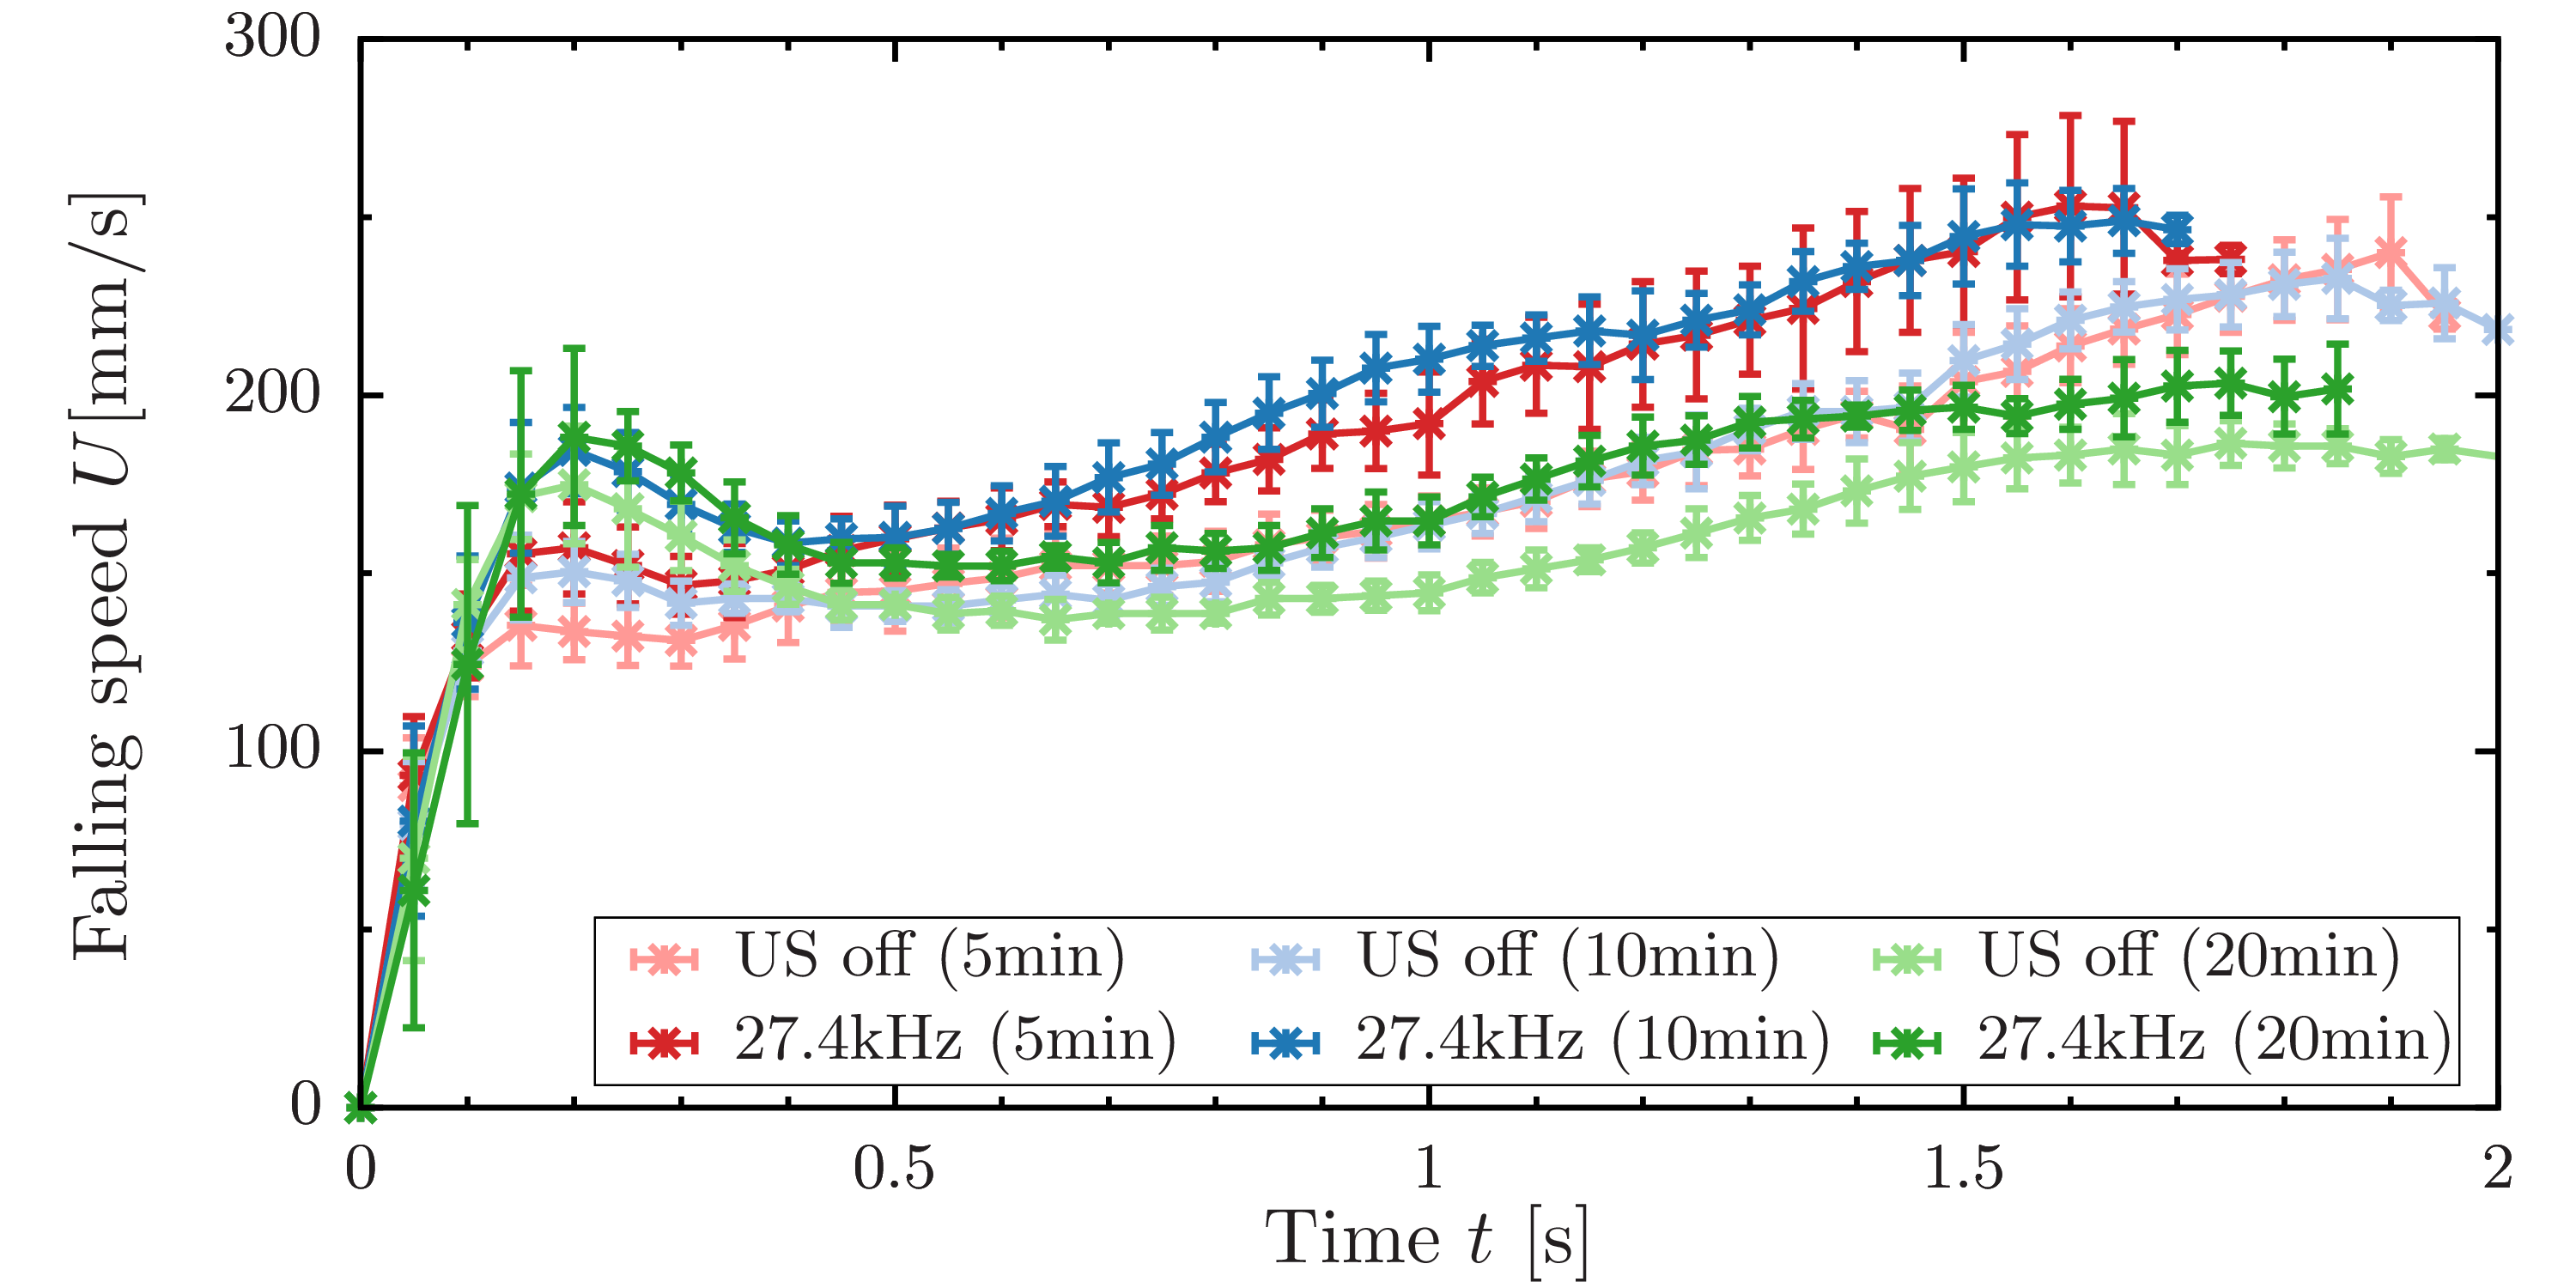
\includegraphics[width=13cm,clip]{5-Discussion/interval.png} 
        \caption{Drop interval change Experimental results.}
        \label{fig:interval-change}
    \end{center}
\end{figure}

\begin{figure}[ht]
    \begin{center}
        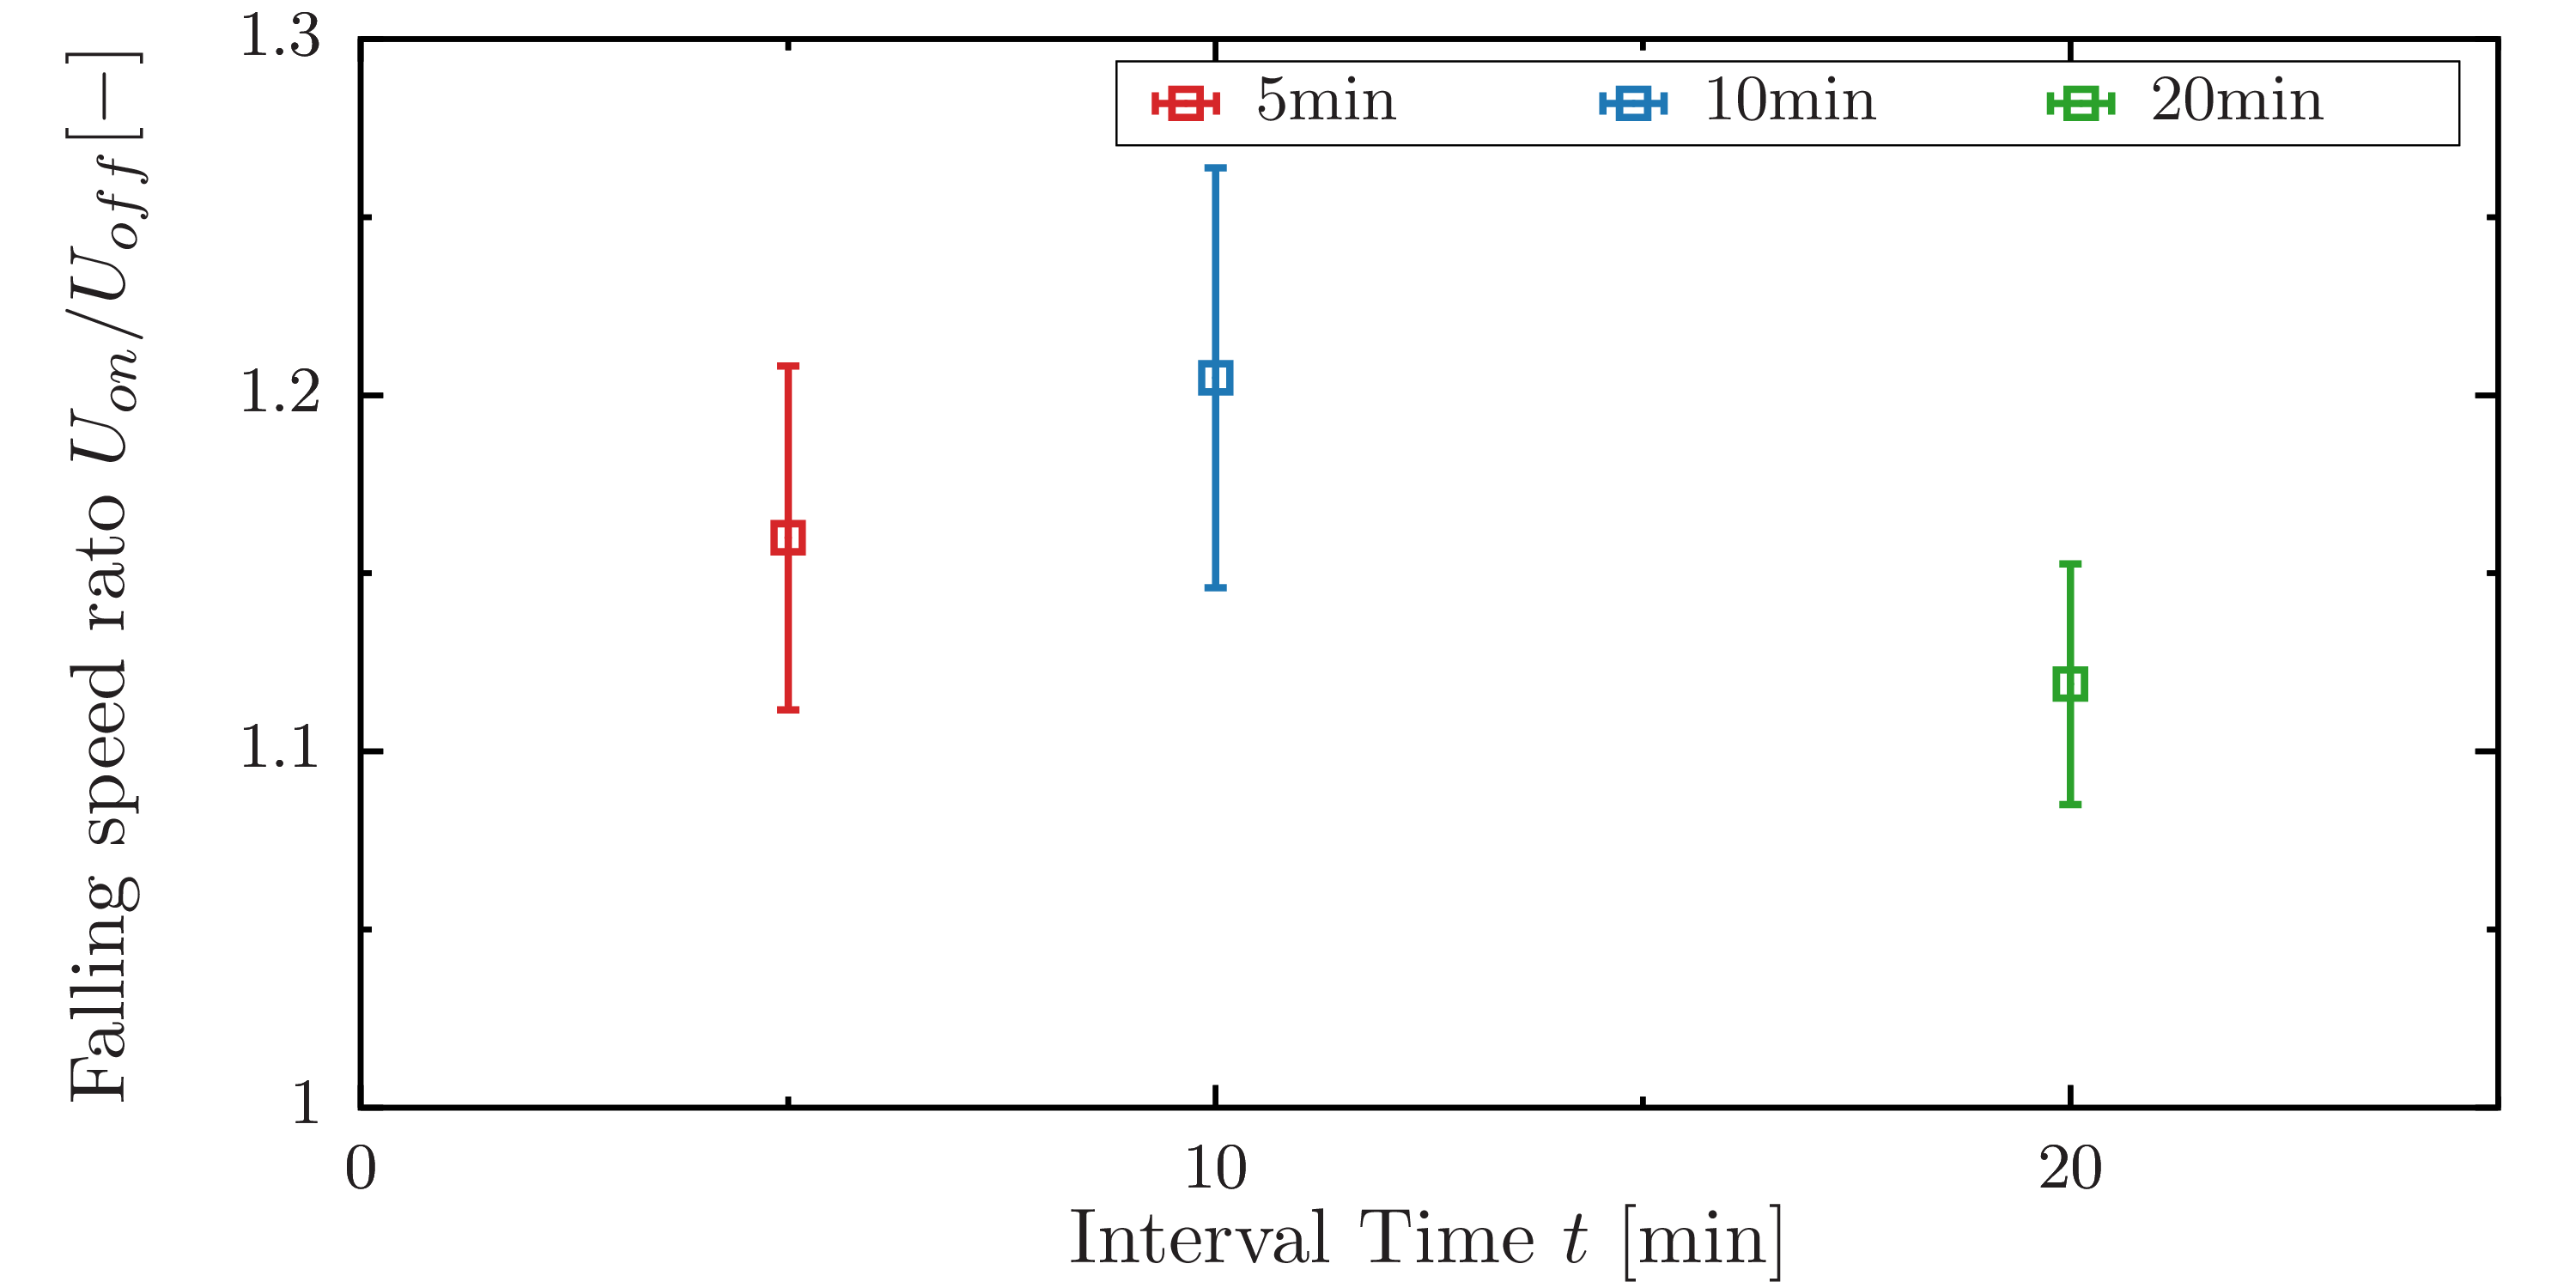
\includegraphics[width=13cm,clip]{5-Discussion/diff.png}
        \caption{Fall velocity ratio due to ultrasound irradiation with change in fall interval.}
        \label{fig:speed-diff}
    \end{center}
\end{figure}

\begin{figure}[ht]
    \begin{center}
        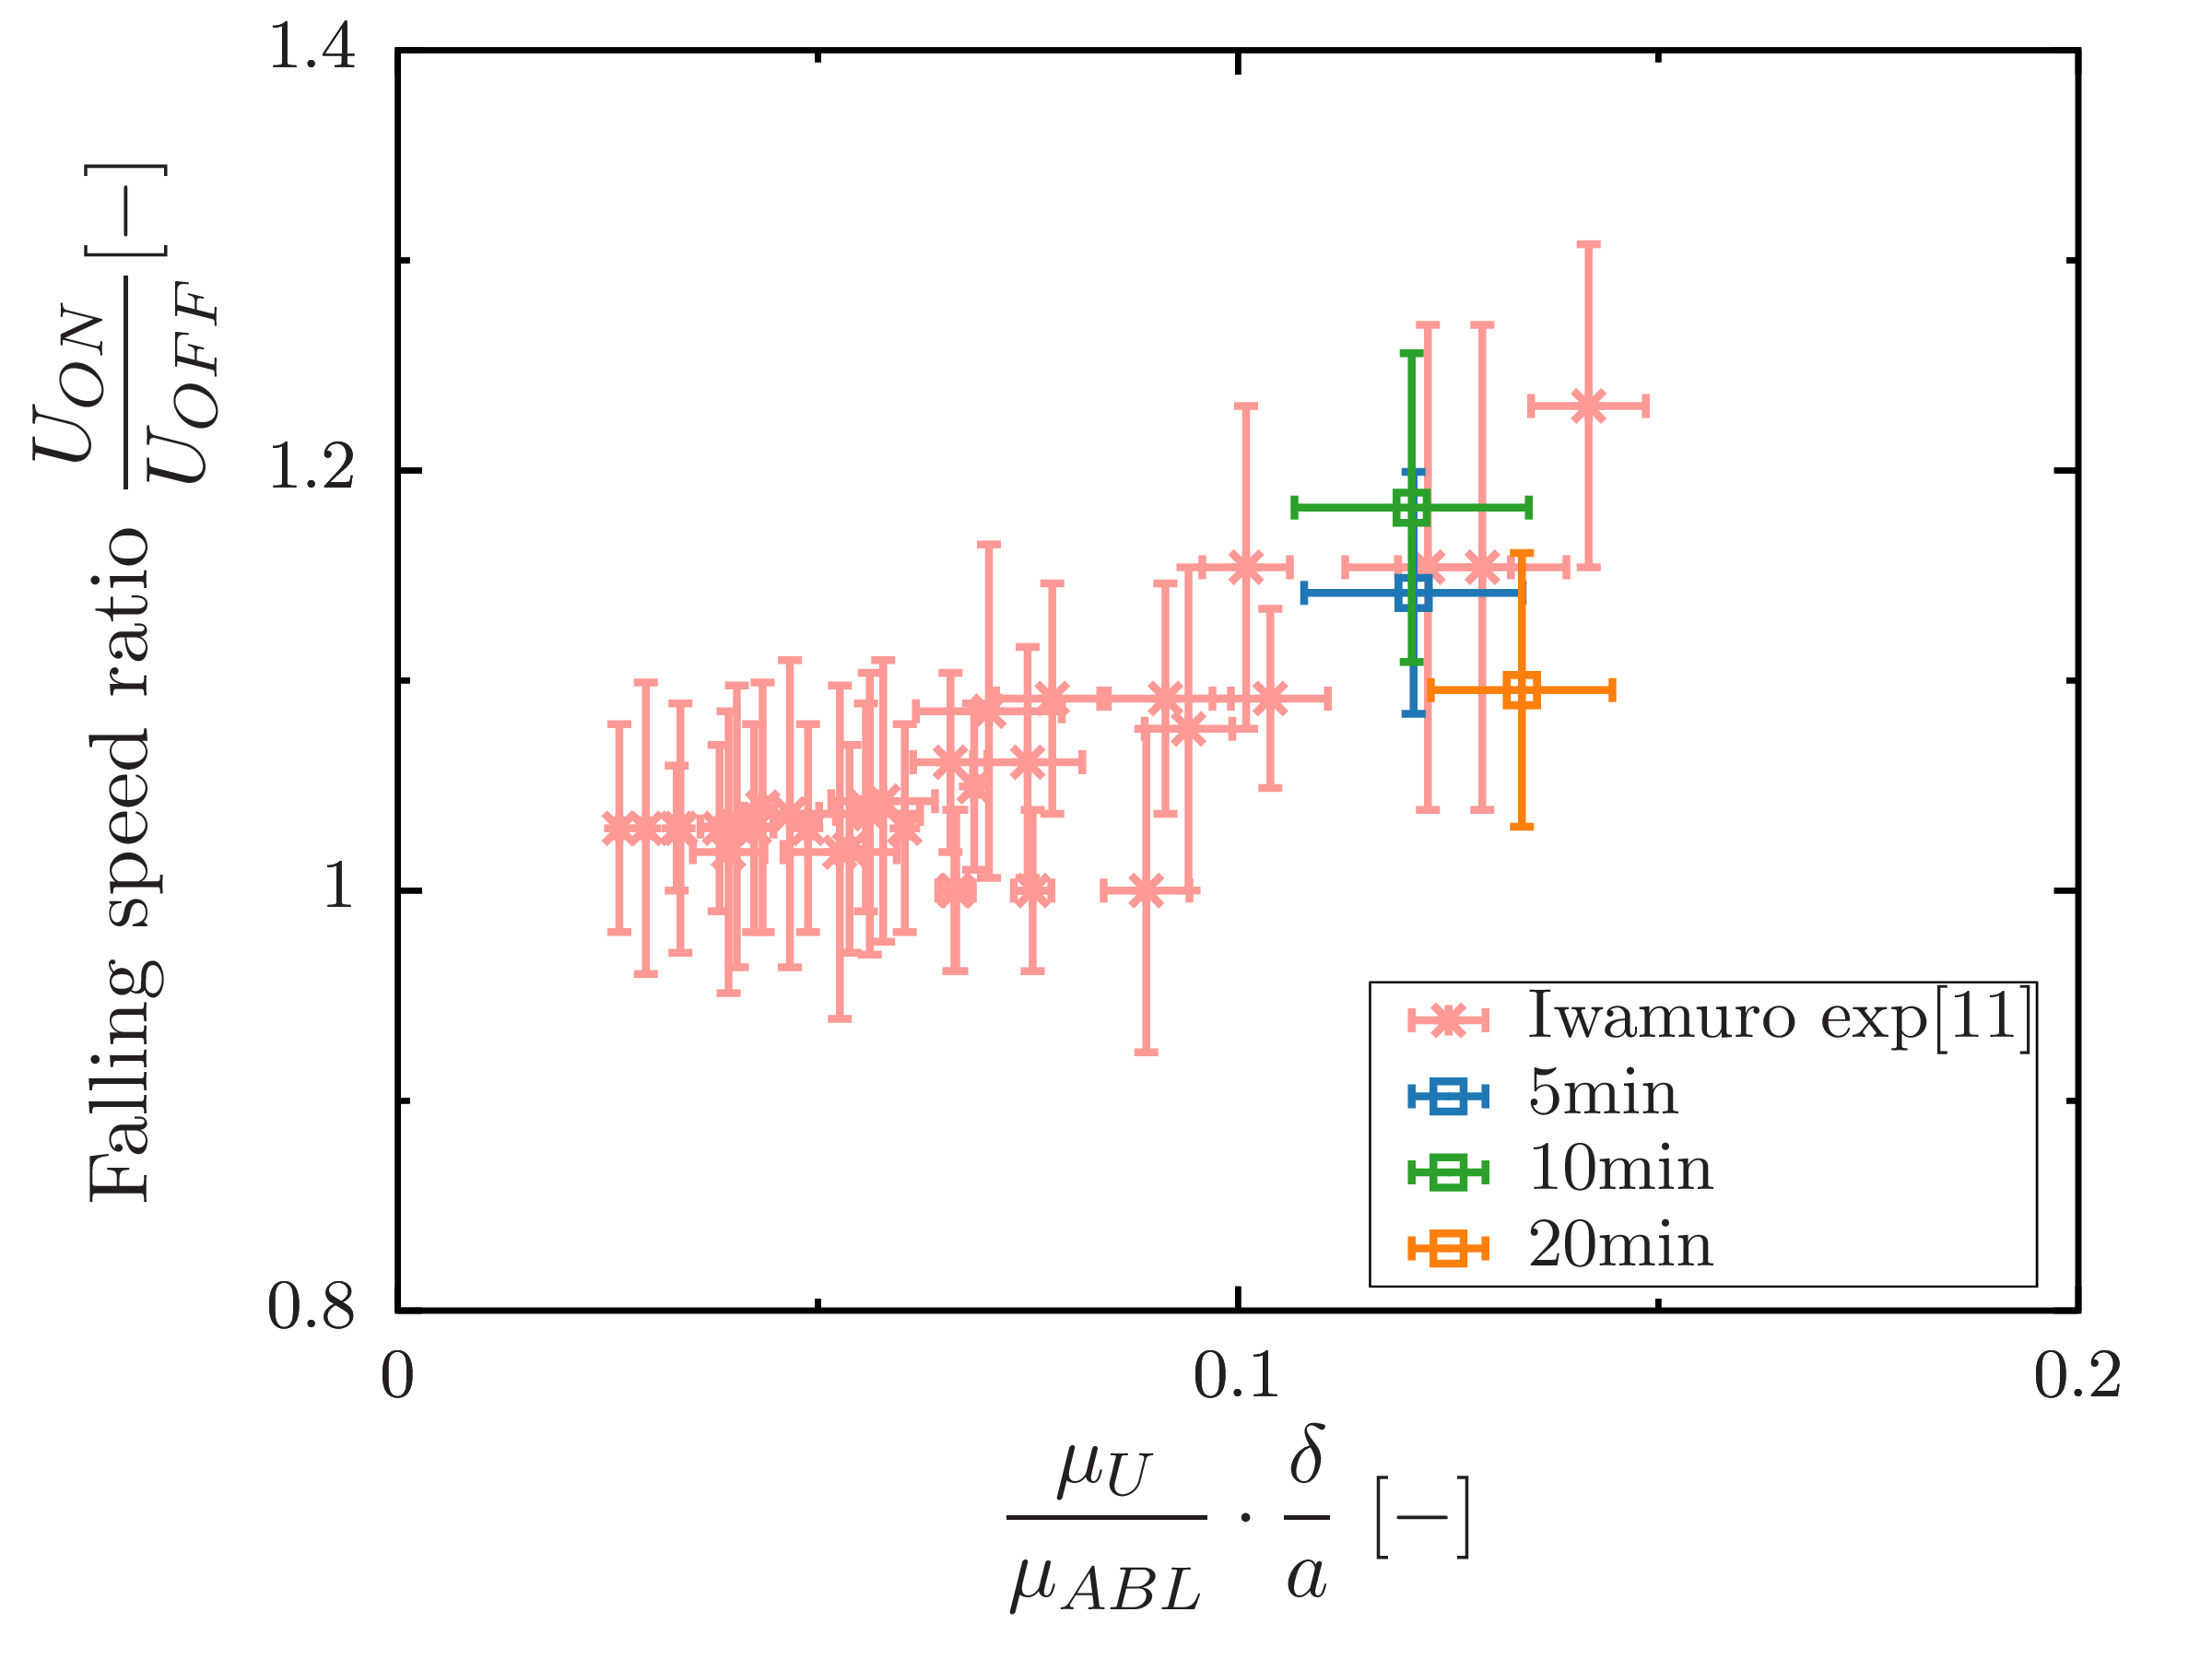
\includegraphics[width=13cm,clip]{5-Discussion/diff-iwamuro.png}
        \caption{Relationship between viscosity and its thickness in the acoustic boundary layer and speed-up by ultrasound irradiation.}
        \label{fig:speed-diff-iwamuro}
    \end{center}
\end{figure}